\section{Конструкторский раздел}

\subsection{Диаграммы состояний (IDEF0)}
На рисунках \ref{fig:idef01} и \ref{fig:idef02} показаны соответственно нулевой и первый уровни диаграммы IDEF0, отображающие процесс мониторинга приоритетов, времени выполнения и простоя процессов.

\begin{figure}[H]
	\centering
	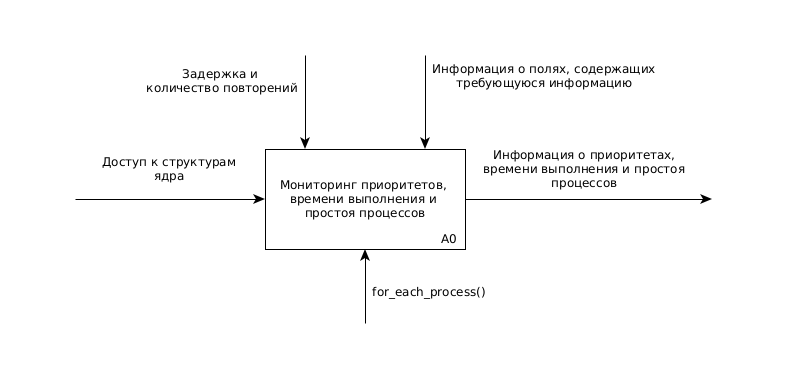
\includegraphics[scale=0.6]{img/idef01.png}
	\caption{IDEF0 нулевого уровня.}
	\label{fig:idef01}
\end{figure}

\begin{figure}[H]
	\centering
	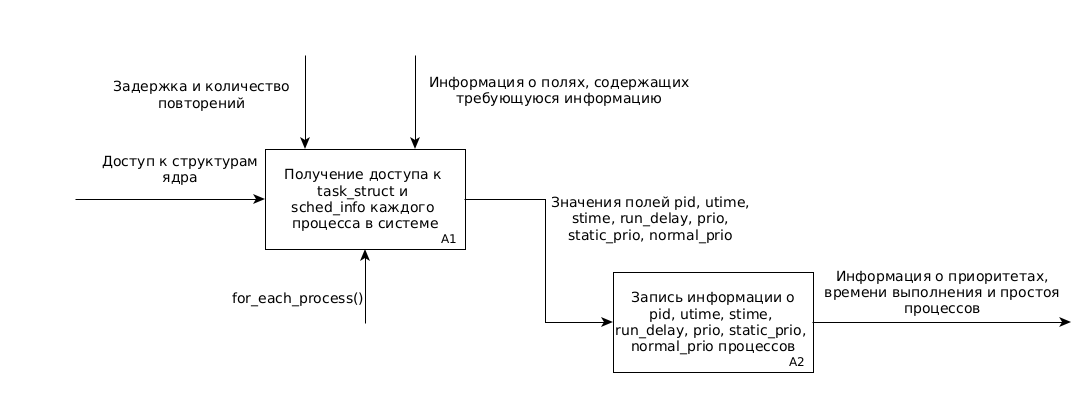
\includegraphics[scale=0.45]{img/idef02.png}
	\caption{IDEF0 первого уровня.}
	\label{fig:idef02}
\end{figure}

\subsection{Алгоритмы определения и логирования приоритетов, времени выполнения и простоя процессов}
На рисунках \ref{fig:read} и \ref{fig:printTasks} представлены алгоритмы определения и логирования приоритетов, времени выполнения и простоя процессов.

\begin{figure}[H]
	\centering
	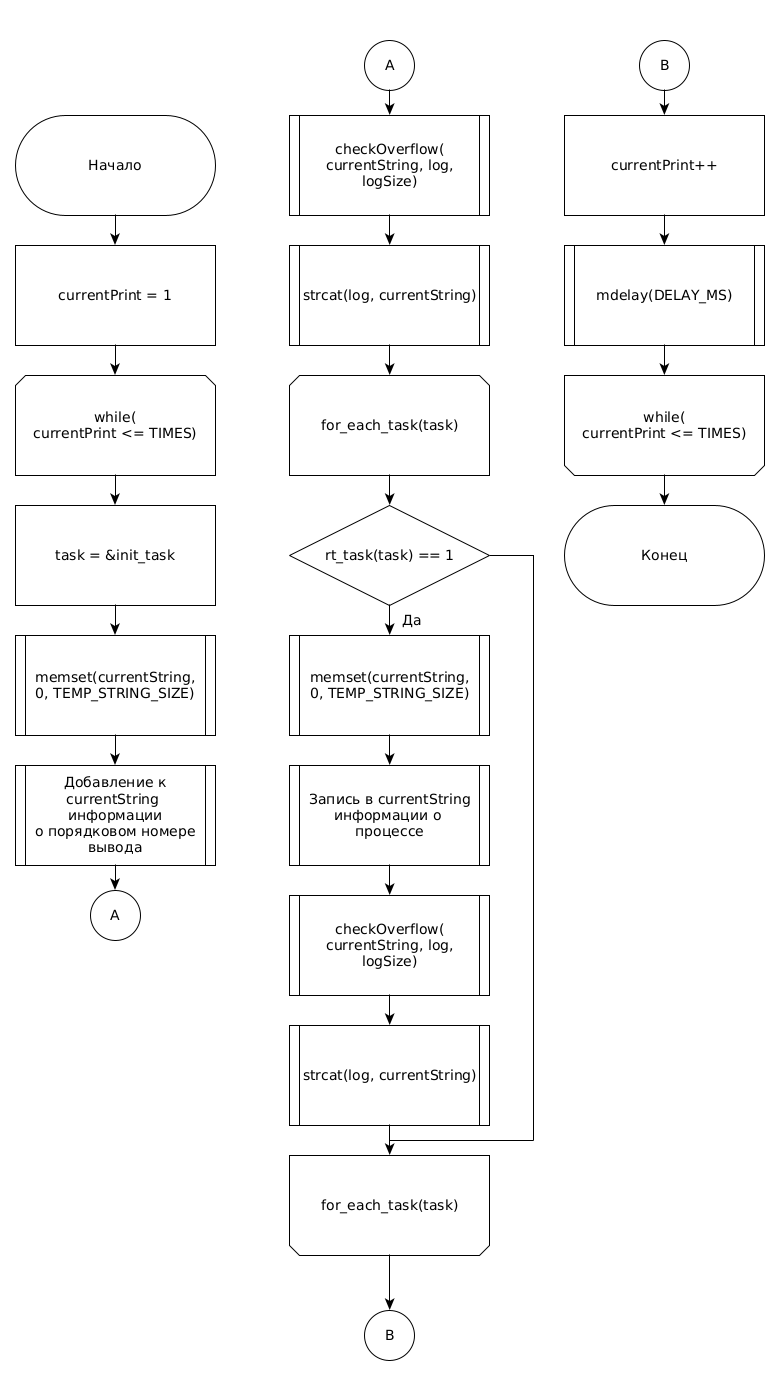
\includegraphics[scale=0.5]{img/printTasks.png}
	\caption{Алгоритм определения приоритетов, времени выполнения и простоя процессов. }
	\label{fig:printTasks}
\end{figure}

\begin{figure}[H]
	\centering
	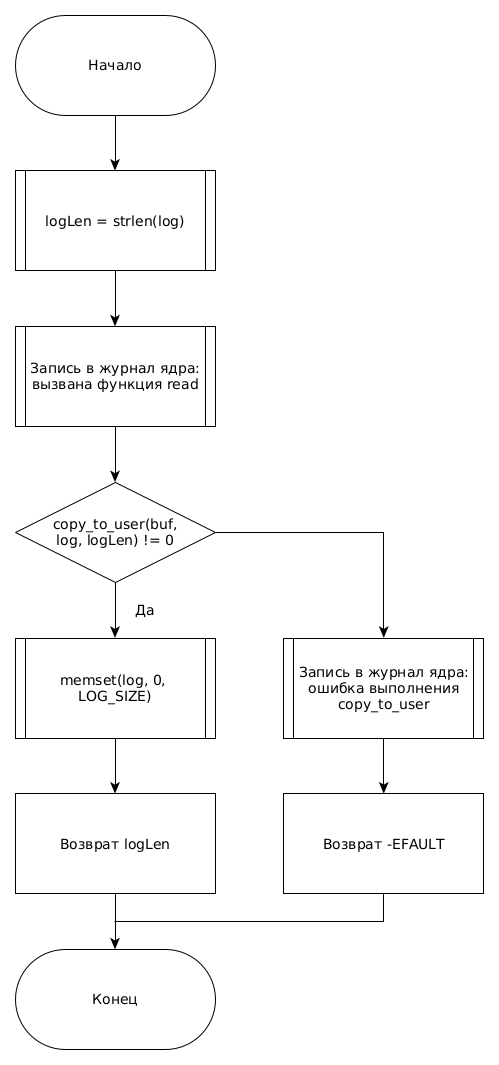
\includegraphics[scale=0.5]{img/yaRead.png}
	\caption{Алгоритм логирования приоритетов, времени выполнения и простоя процессов. }
	\label{fig:read}
\end{figure}

\subsection{Алгоритм предоставления информации о процессах пользователю}
На рисунке \ref{fig:logger} представлен алгоритм предоставления информации о приоритетах, времени выполнения и простоя процессов пользователю.

\begin{figure}[H]
	\centering
	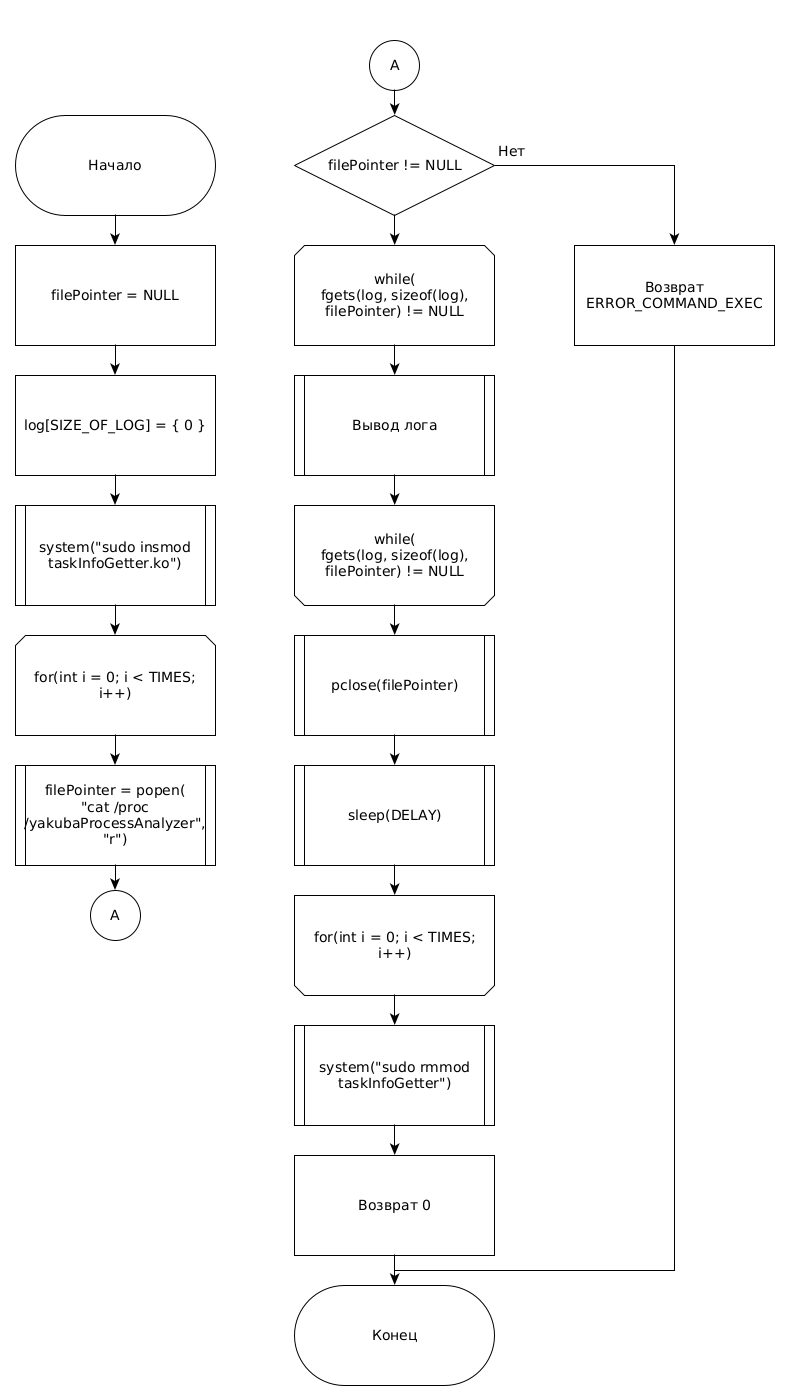
\includegraphics[scale=0.5]{img/starterLogger.png}
	\caption{Алгоритм предоставления информации о приоритетах, времени выполнения и простоя процессов пользователю. }
	\label{fig:logger}
\end{figure}

\subsection{Структура программного обеспечения}
На рисунке \ref{fig:softwareStructure} предоставлена структура программного обеспечения.

\begin{figure}[H]
	\centering
	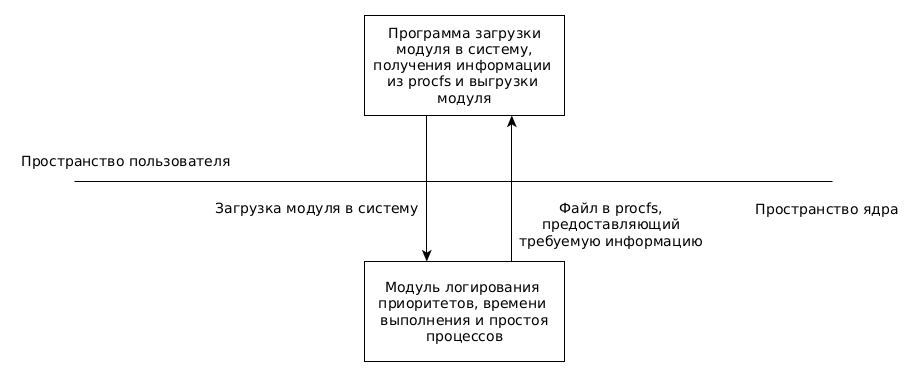
\includegraphics[scale=0.5]{img/softwareStructure.png}
	\caption{Структура программного обеспечения. }
	\label{fig:softwareStructure}
\end{figure}

\pagebreak